\chapter{实验平台}
\section{结构光相机原理}
3D表面成像的一个主要方法是基于结构光的使用,即通过特殊投影仪或由空间光调制器调制的光源对场景进行有源照明,生成具有空间变化的2D结构化照明。结构光图案上每个像素点的强度由数字信号表示。

使用成像传感器来获取受结构光照明下场景的二维图像。如果场景是一个没有任何三维表面变化的平面表面,则所获得图像中显示的模式类似于投影结构光模式。然而,当场景中的表面是非平整面时,从相机看到的投影结构光模式会被表面的几何形状扭曲。 结构光3D表面成像技术原理在于基于从投影结构光模式失真信息提取3D表面形状。可以使用各种结构光原理和算法计算出场景中物体的精确3D表面轮廓。成像传感器、结构光投影仪和物体表面点之间的几何关系如图\ref{fig:3d-camera}所示。\cite{gengStructuredlight3DSurface2011,salviStateArtStructured2010}


% 可以用三角测量原理表示,如式

% \begin{equation}
%   R=B \frac{\sin (\theta)}{\sin (\alpha+\theta)}
% \end{equation}

\begin{figure}[htbp]
  \centering
  \includegraphics[width=0.5\textwidth]{figures/2/3d-camera.pdf}
  \caption{结构光测距原理示意图}\label{fig:3d-camera}
\end{figure}

三角测量式三维成像的关键在于区分出二维投影获取的图像中的单个投射光斑。根据投射光源可将其分二值编码、彩色编码、光栅条纹编码等。其中,光栅条纹编码最常见,它具有高精度、快速等优势。\cite{vanderjeughtRealtimeStructuredLight2016}在使用光栅条纹技术的结构光相机进行高度测量时,通常先采取四步相移、多频外差等方法获取样本表面高度的绝对相位调制,然后基于三角测量原理进行计算。\cite{wangGuangzhajiegouguangxitongceliangwuchayunihejingduyanjiu2020}

相移法是一种用于三维表面成像的著名条纹投影方法。一组正弦波图案被投射到物体表面上。平面上任一像素位置处接收的光强$I_{n}(x, y)$可由式\ref{equ:in}表示

\begin{equation}\label{equ:in}
  I_{n}(x, y)=I_{mod}(x,y) \cos \left(\varphi(x, y)+\delta_{n}\right)+I_{0}(x,y)
\end{equation}


其中$I_{mod}(x,y)$是振幅,$\varphi(x, y)$是像素点的相位,$\delta_{n}$ 是每次拍摄时移动的相位,这个三个变量组成的$I_{mod}(x,y) \cos \left(\varphi(x, y)+\delta_{n}\right)$是系统投射的余弦调制光强(交流成分);$I_{0}(x,y)$是直流成分,即环境光强。根据N步相位法,$\delta_{n}=\frac{2 \pi(n-1)}{N}, n=1,2, \cdots, N$ ,而上式有三个未知量,因此N >= 3,即通过三幅或三幅以上投影可求解未知相位,相位计算公式如式\ref{equ:varphical}所示。

\begin{equation}\label{equ:varphical}
  \varphi(x, y)=\arctan \left(\frac{\sum_{n=1}^{N} I_{n}(x, y) \cos \left(\frac{2 n \pi}{N}\right)}{\sum_{n=1}^{N} I_{n}(x, y) \sin \left(\frac{2 n \pi}{N}\right)}\right)
\end{equation}


根据测量相位$\varphi(x, y)$和参考平面的相位值之间的差异按式\ref{equ:distance}可以计算出3D坐标。

\begin{equation}\label{equ:distance}
  h=\frac{L \times x_{A C}}{d+x_{A C}}=\frac{L \times P_{0} \times \varphi_{A C}}{2 \pi d+P_{0} \times \varphi_{A C}}
\end{equation}


其中L表示系统与基准平面的距离,d表示相机与投影仪之前的基线距离,$P_{0}$ 表示投影光栅条纹的周期, $\varphi_{A C}$为相位差。




\section{硬件平台}

实验硬件平台主要包括结构光相机、协作机器人、工控机和GPU服务器。结构光相机用于采集样本,是视觉方案中最重要的提供输入的传感器。协作机器人用于挂载结构光相机执行运动指令。工控机用于运行自动数据采集程序。GPU服务器负责对采集数据进行处理并进行缺陷检测输出结果。

\subsection{传感器设备}
\begin{figure}[htbp]
  \centering
  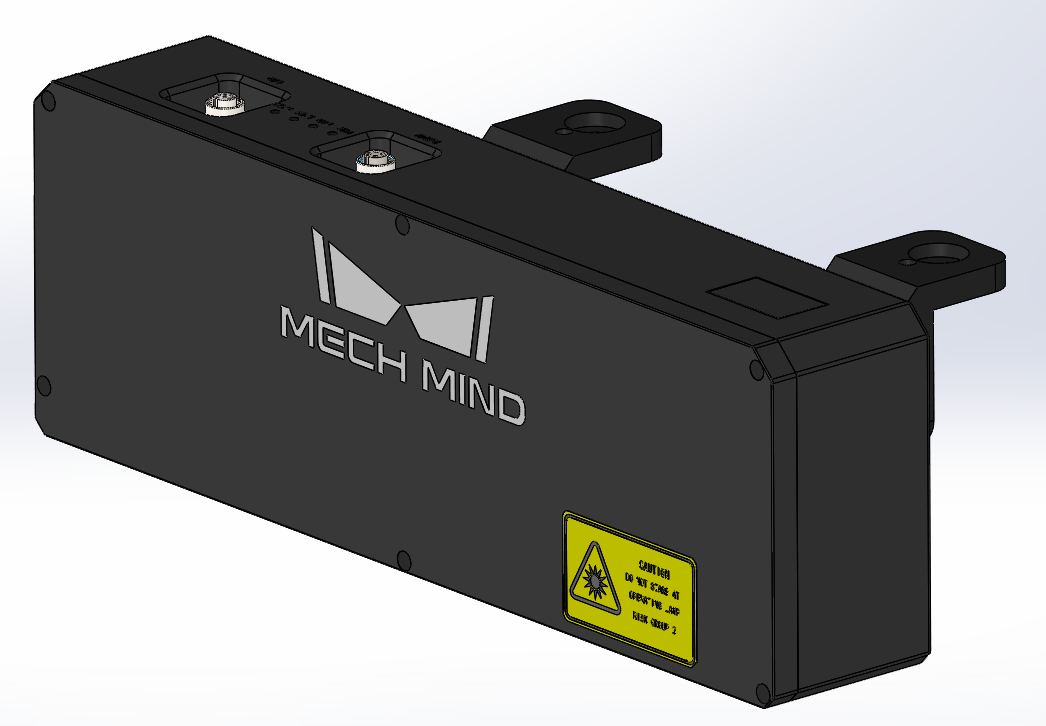
\includegraphics[width=0.5\textwidth]{figures/2/Mech-Eye-V3.png}
  \caption{梅卡曼德Mech-Eye PRO M 工业级3D相机}\label{fig:Mech-Eye-V3}
\end{figure}
本文采用梅卡曼德的PRO M高性能工业级3D相机作为视觉传感器搭建系统,如图\ref{fig:Mech-Eye-V3}所示。该相机使用蓝光作为结构光光源,能够采集被检物体表面的深度信息以及RGB色彩信息,可以直接输出ply格式的无序点云数据、具有RGB通道的彩色图像和tiff格式的单通道深度图像。此外,该相机具有精度高,速度快,抗环境光性能优异,运行稳定的优点,其部分参数如表\ref{tab:category}所示。其中1m到2m的推荐工作距离与AUBO-E5协作机器人的工作区域匹配,能覆盖本文实验所用的工业产品;1920 × 1200的分辨率和2.3MP的像素数表示其能输出高清晰度的RGB图像;0.2mm @ 2m的Z向单点重复精度则表示其能提供高精度的深度图。
\begin{table}[htbp]
  \centering
  \caption{结构光相机部分重要参数} \label{tab:category}
  \begin{tabular*}{0.75\textwidth}{@{\extracolsep{\fill}}cccc}
  \toprule
    指标			&参数		 \\
  \midrule
    工作距离范围$(mm)$ &  $1000\sim 2000$    \\
    分辨率			&$1920\times 1200$		 \\
    像素数$(MP)$	&$2.3$	 \\
    Z向单点重复精度$(\sigma)$	& $0.05mm @ 1m$\\
    典型采集时间$(s)$	& $0.6\sim0.9$\\
    基线长度$(mm)$ &  $68$    \\
    光源$(mm)$ &  蓝光LED$(459nm,RG2)$    \\
  \bottomrule
  \end{tabular*}
\end{table}


\subsection{协作机器人}

本文使用AUBO-E5协作机器人挂载结构光相机,并接收工控机自动数据采集程序的指令进行运动,实现智能化采集大量多视角的样本数据,为后续缺陷检测任务服务。AUBO-E5协作机器人由机械臂、控制柜和示教器共同组成。机械臂具有6自由度,能够负载5kg,其臂展有1008mm,最大工作半径886.5mm,重定位精度达到0.02mm,能够满足在实验室中轻量化作业需求。示教器作为人机交互工具,具有显示器,提供可视化界面操作机械臂。协作机器人如图\ref{fig:aubo}所示,左图为机械臂,右图为示教器。
\begin{figure}[htbp]
  \centering
  \begin{subfigure}
      \centering
      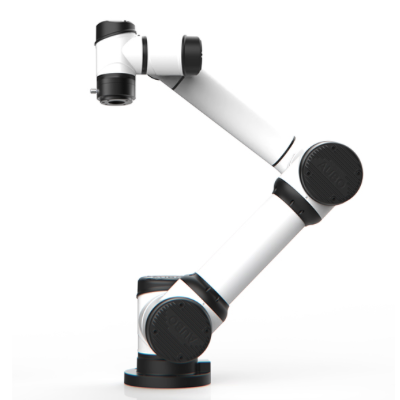
\includegraphics[width=.35\linewidth]{figures/2/aubo-1.png}  
    \end{subfigure}
    \begin{subfigure}
      \centering
      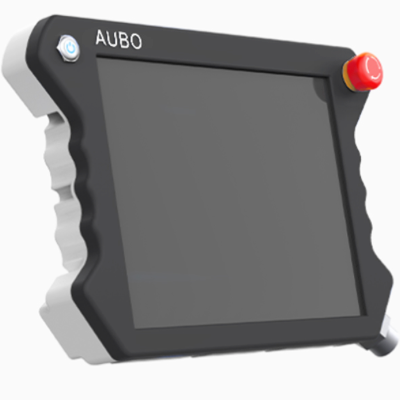
\includegraphics[width=.35\linewidth]{figures/2/aubo-2.png} 
    \end{subfigure}
  \caption{AUBO-E5协作机器人}
  \label{fig:aubo}
\end{figure}



\subsection{计算单元}
本文使用的运行缺陷检测算法程序服务器硬件上搭载了英伟达RTX3090型号的GPU,具有10496个CUDA核以及24GB的GDDR6X类型显存;CPU使用的是AMD EPYC 74F3,具有24核48线程,基础频率3.2GHz。

\begin{figure}[htbp]
  \centering
  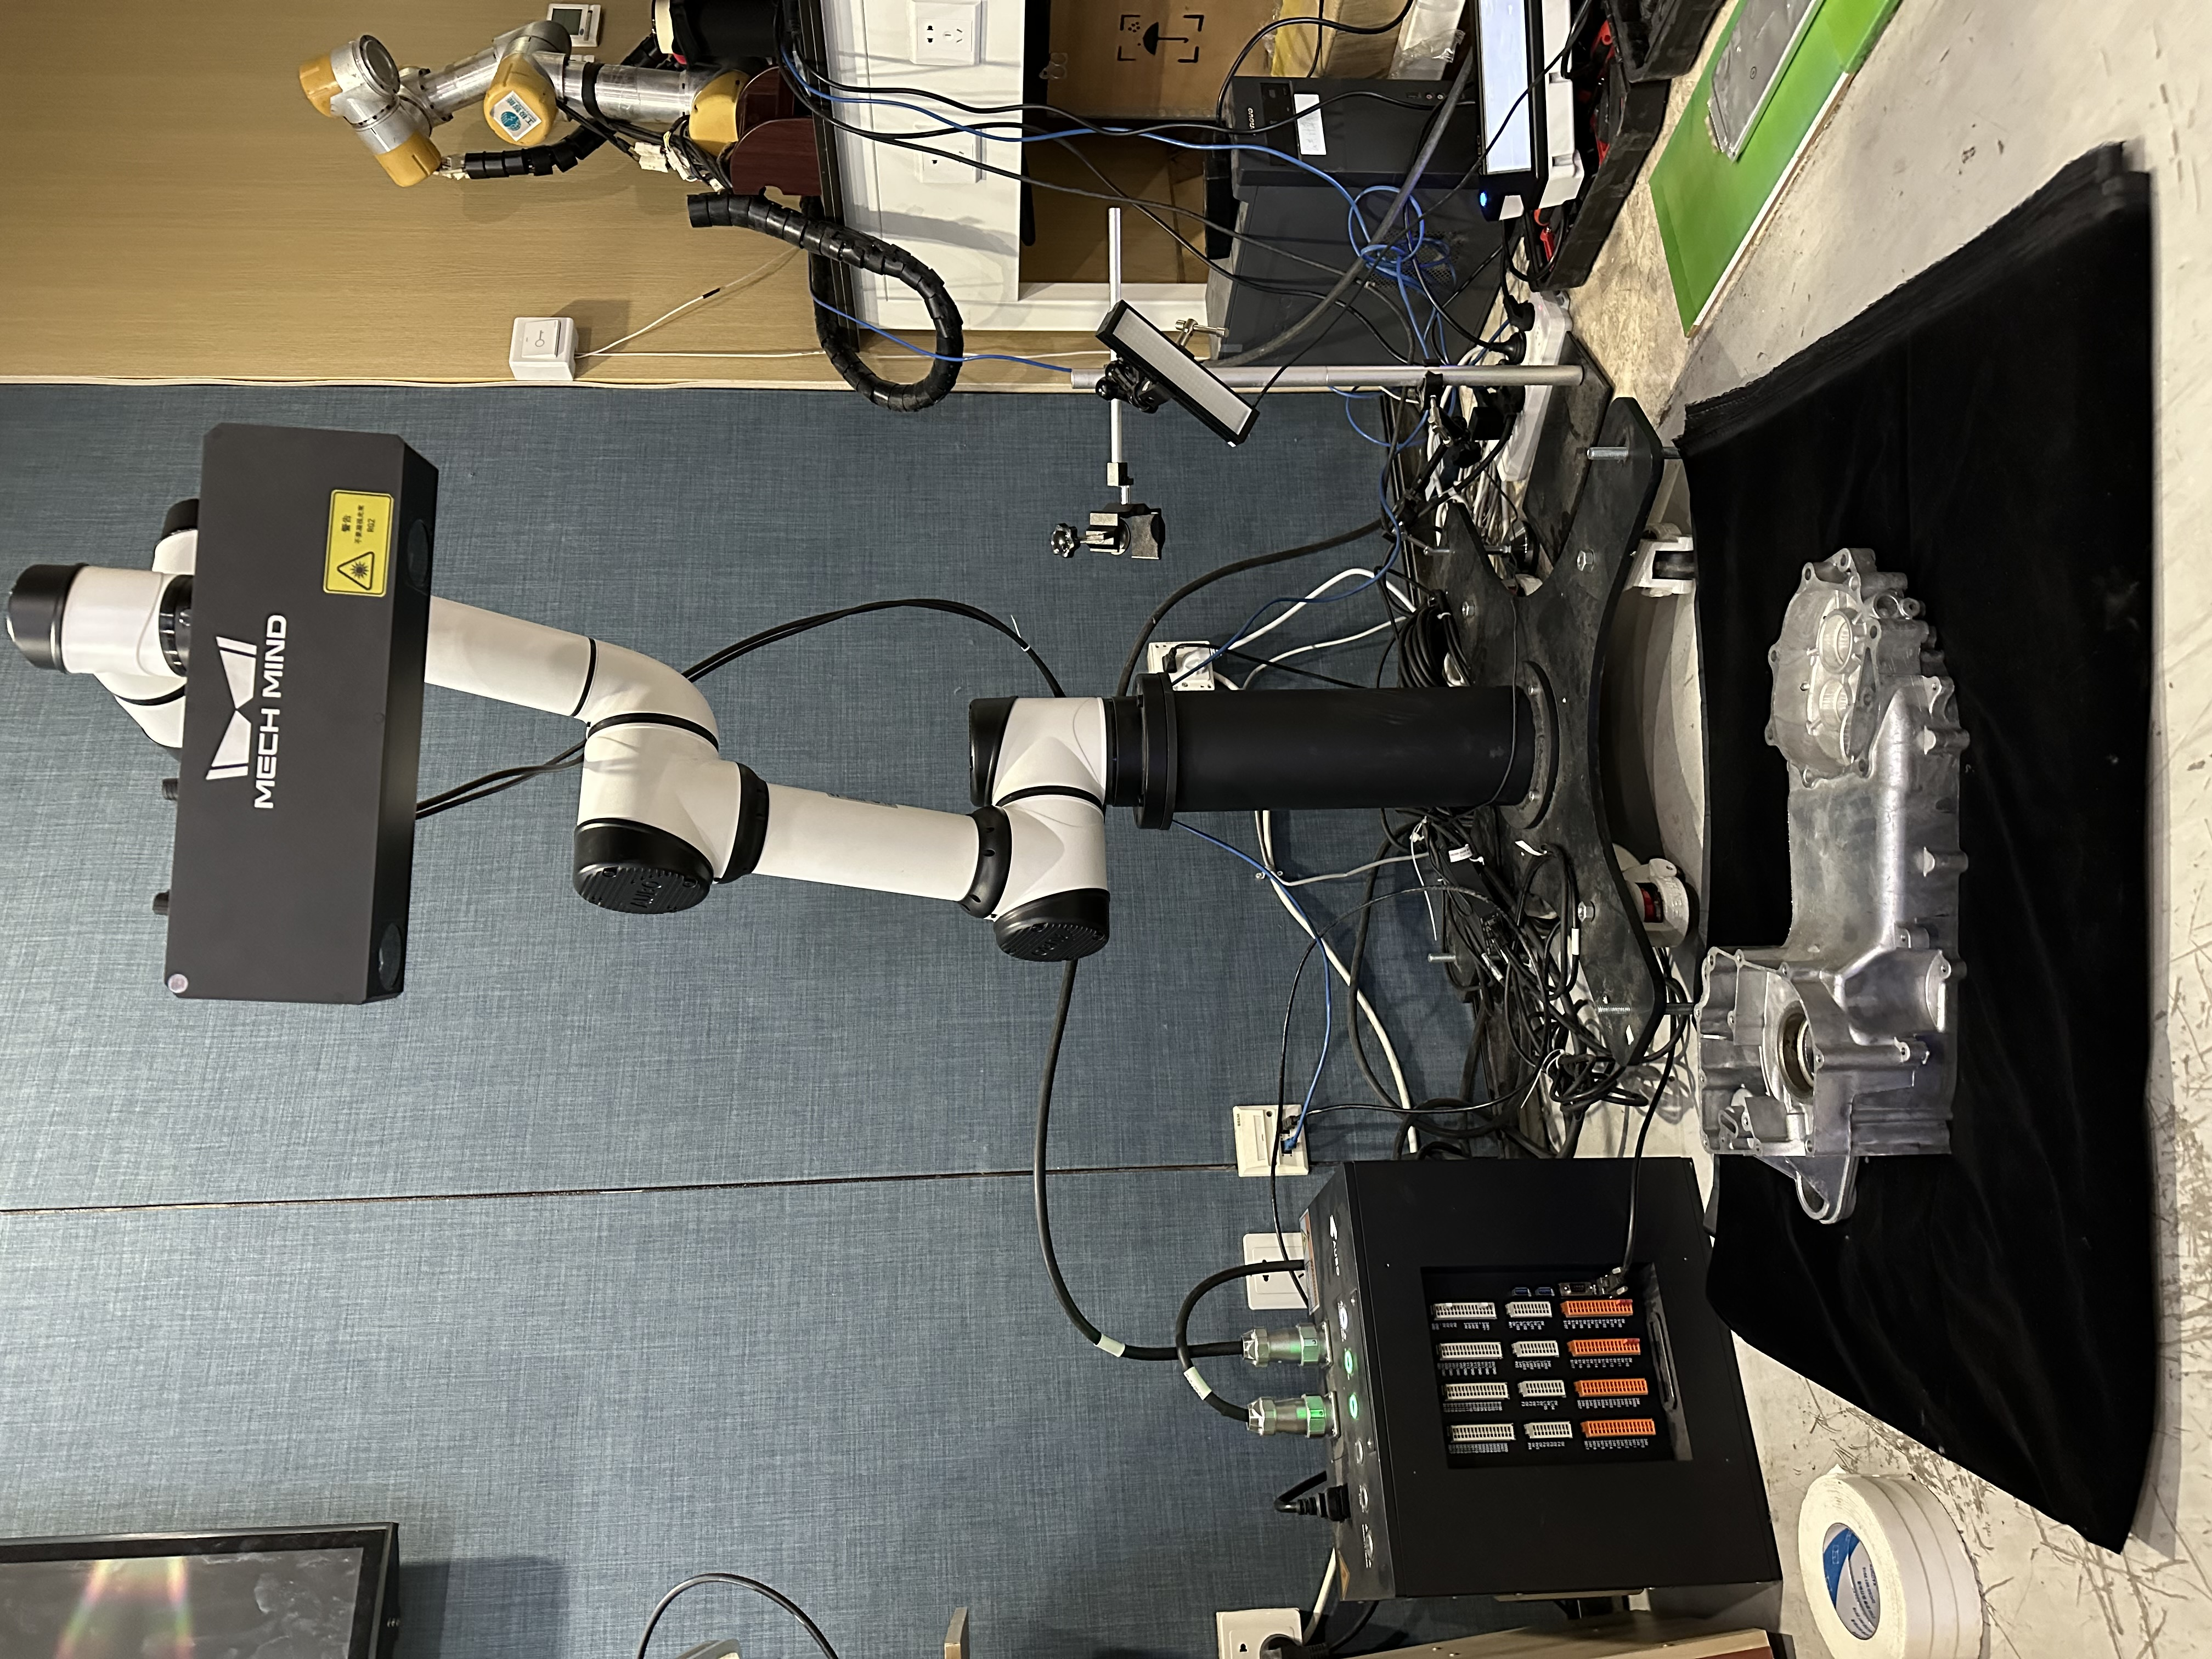
\includegraphics[width=0.5\textwidth,angle=270]{figures/2/hw-platform.jpeg}
  \caption{缺陷检测实验硬件平台}\label{fig:hw-platform}
\end{figure}
本文在实验室组合以上硬件设备搭建的实验硬件平台如图\ref{fig:hw-platform}所示,环境光源为室内灯光,存在直射光源干扰。实验平台的感知系统由协作机器人、结构光相机和模拟工作台共同组成,采集指令和采集数据存储由工控机处理。实验平台的设计目标是自动化采集样本数据,实现仅依靠正常样本的缺陷检测。本文的实验对象为工作区内的工业产品,针对不同场景,本文采集不同的数据并使用不同方法进行处理,实现被检物的缺陷检测。


\section{软件平台}
本文使用的工控机系统环境为Ubuntu18.04,主要使用的库包括GUI库Qt、点云处理库PCL和Open3D、外设SDK(相机和机械臂)和深度学习训练框架Pytorch等。

Qt是一个跨平台的C++应用程序开发框架,可以用来开发GUI程序。在本文的人机交互界面中,我们使用了Qt Creator IDE进行开发,该IDE提供了可视化编辑UI界面的功能。

PCL(Point Cloud Library)和Open3D都是点云处理库,PCL是基于C++11标准的模块化库,Open3D是基于Python的模块化库。两者都可以对点云数据进行读取、可视化以及滤波,针对特征提取等高阶用法,两者提供的方法有所区别。由于Open3D基于Python,其对深度学习模型的支持较好,适合在模型训练阶段快速试验;而PCL基于采用C++,对于大量数据处理其优势显现,因此本文根据实际阶段应用两者。

PyTorch是一个开源的深度学习框架,使用动态计算图,方便灵活调试。此外,Pytorch可以利用NVIDIA的CUDA和cuDNN库,轻松地将计算任务切换到GPU上以获得更快的运行速度。

梅卡曼德在官方网站提供了本文所选型号相机的SDK(软件开发套件),包括面向Windows平台和Linux平台的C++、Python和C\#版本,可以方便部署到工控机和嵌入式终端。Windows版本SDK还包含一个GUI可视化配置相机参数和手动采集数据的应用,方便实验前期对相机进行观察调整。

AUBO协作机器人支持通过示教器进行简易编程,同时也在其官网提供了Linux平台的C++和Python版本的SDK。综合考虑性能和兼容性,C++版本SDK作为本文开发相机和机器人的首选。

\section{相机标定}
3D成像技术的一个重要组成部分是相机和投影仪校准技术,这在建立3D成像系统的测量精度方面起着至关重要的作用。

由于大多数3D成像系统使用2D光学传感器,因此相机校准程序建立了一个像素在2D图像上(在相机坐标系中)和一条直线在3D空间中(世界坐标系中)的关系,沿着这条直线定位物体点,并根据实际情况考虑镜头畸变。通常使用简化的相机模型和一组内部参数来描述这些关系。校准方法通常需要已知校准对象的多个角度和距离的图像。平面棋盘格模式是经常使用的校准对象,因为它非常容易制作,可以用标准打印机打印,并且具有易于检测的独特角落。

\subsection{相机校准算法}

相机参数包括内参、外参和畸变系数。要估计相机参数,需要有三维世界点及其对应的二维图像点。Matlab的针孔校准算法基于Jean-Yves Bouguet提出的模型。该模型包括针孔相机模型\cite{zhangFlexibleNewTechnique2000}和镜头畸变\cite{heikkilaFourstepCameraCalibration1997}。针孔相机模型不考虑镜头畸变,因为理想的针孔相机没有镜头。为了准确地表示真实相机,算法使用的完整相机模型包括径向和切向镜头畸变。

针孔相机是一种简单的相机模型,其没有镜头,只有一个小孔。光线通过小孔并在相机的对面投射出倒置的图像。将虚像平面视为在相机前方,并包含场景的正立图像。

针孔相机参数用一个$3\times4$矩阵表示,称为相机矩阵P,该矩阵将三维世界场景映射到图像平面上。校准算法使用外参和内参参数计算相机矩阵。

\begin{equation}
  P=K\begin{bmatrix}
    R & t
  \end{bmatrix}
\end{equation}


K是内参,包括焦距、光学中心(也称为主点)和倾斜系数,表示从三维世界坐标系到三维相机坐标系的刚性变换。相机内部矩阵K的定义如下:

\begin{equation}
  K = \left[\begin{array}{ccc}f_{x} & s & c_{x} \\0 & f_{y} & c_{y} \\0 & 0 & 1\end{array}\right]
\end{equation}

其中$(c_{x},c_{y})$是光学中心,单位是像素;$(f_{x},f_{y})$是像素单位焦距,s是倾斜系数,当图像轴不垂直是为非零。

像素焦距可以通过世界单位中的焦距F计算而得,$(p_{x},p_{y})$为像素在世界单位的大小,世界单位通常用mm表示。

\begin{equation}
  \left\{\begin{array}{l}f_{x}=\frac{F} {p_{x}} \\f_{y}=\frac{F} {p_{y}} \end{array}\right.
\end{equation}



[R t]是外参,包括相机在三维场景中的旋转R和平移t,表示从三维相机坐标系到二维图像坐标系的投影变换。

相机坐标系的原点位于其光学中心,其x轴和y轴定义了图像平面。世界坐标通过外参转换为相机坐标。相机坐标再利用内参映射到图像平面上。

\begin{equation}
  \mathrm{W}\left[\begin{array}{l}x \\y \\1\end{array}\right]=P\left[\begin{array}{l}X \\Y \\Z \\1\end{array}\right]
\end{equation}


其中w是缩放系数,(x,y)是图像像素的坐标,(X,Y,Z)是真实世界中的坐标。

\subsection{投影仪的校准}

投影仪的校准有两个方面:作为主动光源,需要校准投影仪的强度以恢复其照明强度的线性关系;同时作为反向相机,也需要像普通相机一样进行几何校准。

首先是投影仪的强度校准。为了增强对比度,投影仪的强度曲线通常会通过伽马变换进行调整。当在3D成像系统中作为主动光源使用时,需要进行校准以恢复照明强度的线性关系。为此,需要投射出几个测试图案,并由成像传感器捕获这些图案。可以建立实际投射图案和图像像素值之间的关系,并将其拟合为高阶多项式函数。然后计算反函数并用于修正在3D成像过程中要投射的模式。

然后是投影仪的几何校准。将投影仪视为反向相机;投影仪的光学模型与相机相同,它们之间唯一的区别是投射方向。反向模型使得在2D图像上(在相机坐标系下)关联一个像素和3D空间中的一条直线(世界坐标系下)变得困难,因为我们无法确定给定点在3D空间中会被投影到哪个位置。 投影仪校准的关键问题是如何建立对应关系。 一旦建立了对应关系,就可以使用摄像机校准算法来校准投影仪。

投影仪校准是通过使用预校准相机和校准平面来完成的。首先,在相机坐标系中恢复出校准平面。然后,投射并捕获校准图案。可以通过将捕获的图像上的角点重新投影到平面板上来确定在校准平面上形成的棋盘格模式的角点的三维坐标,因为相机与平面板之间的空间关系已经恢复。最后,可以使用获取到的点对应关系来对投影仪进行校准。这种方法在理论上很简单,并且实现起来相对容易。但是,这些方法的校准精度严重依赖于相机预先校准的精度。

\section{数据自动采集应用}
\begin{figure}[htbp]
  \centering
  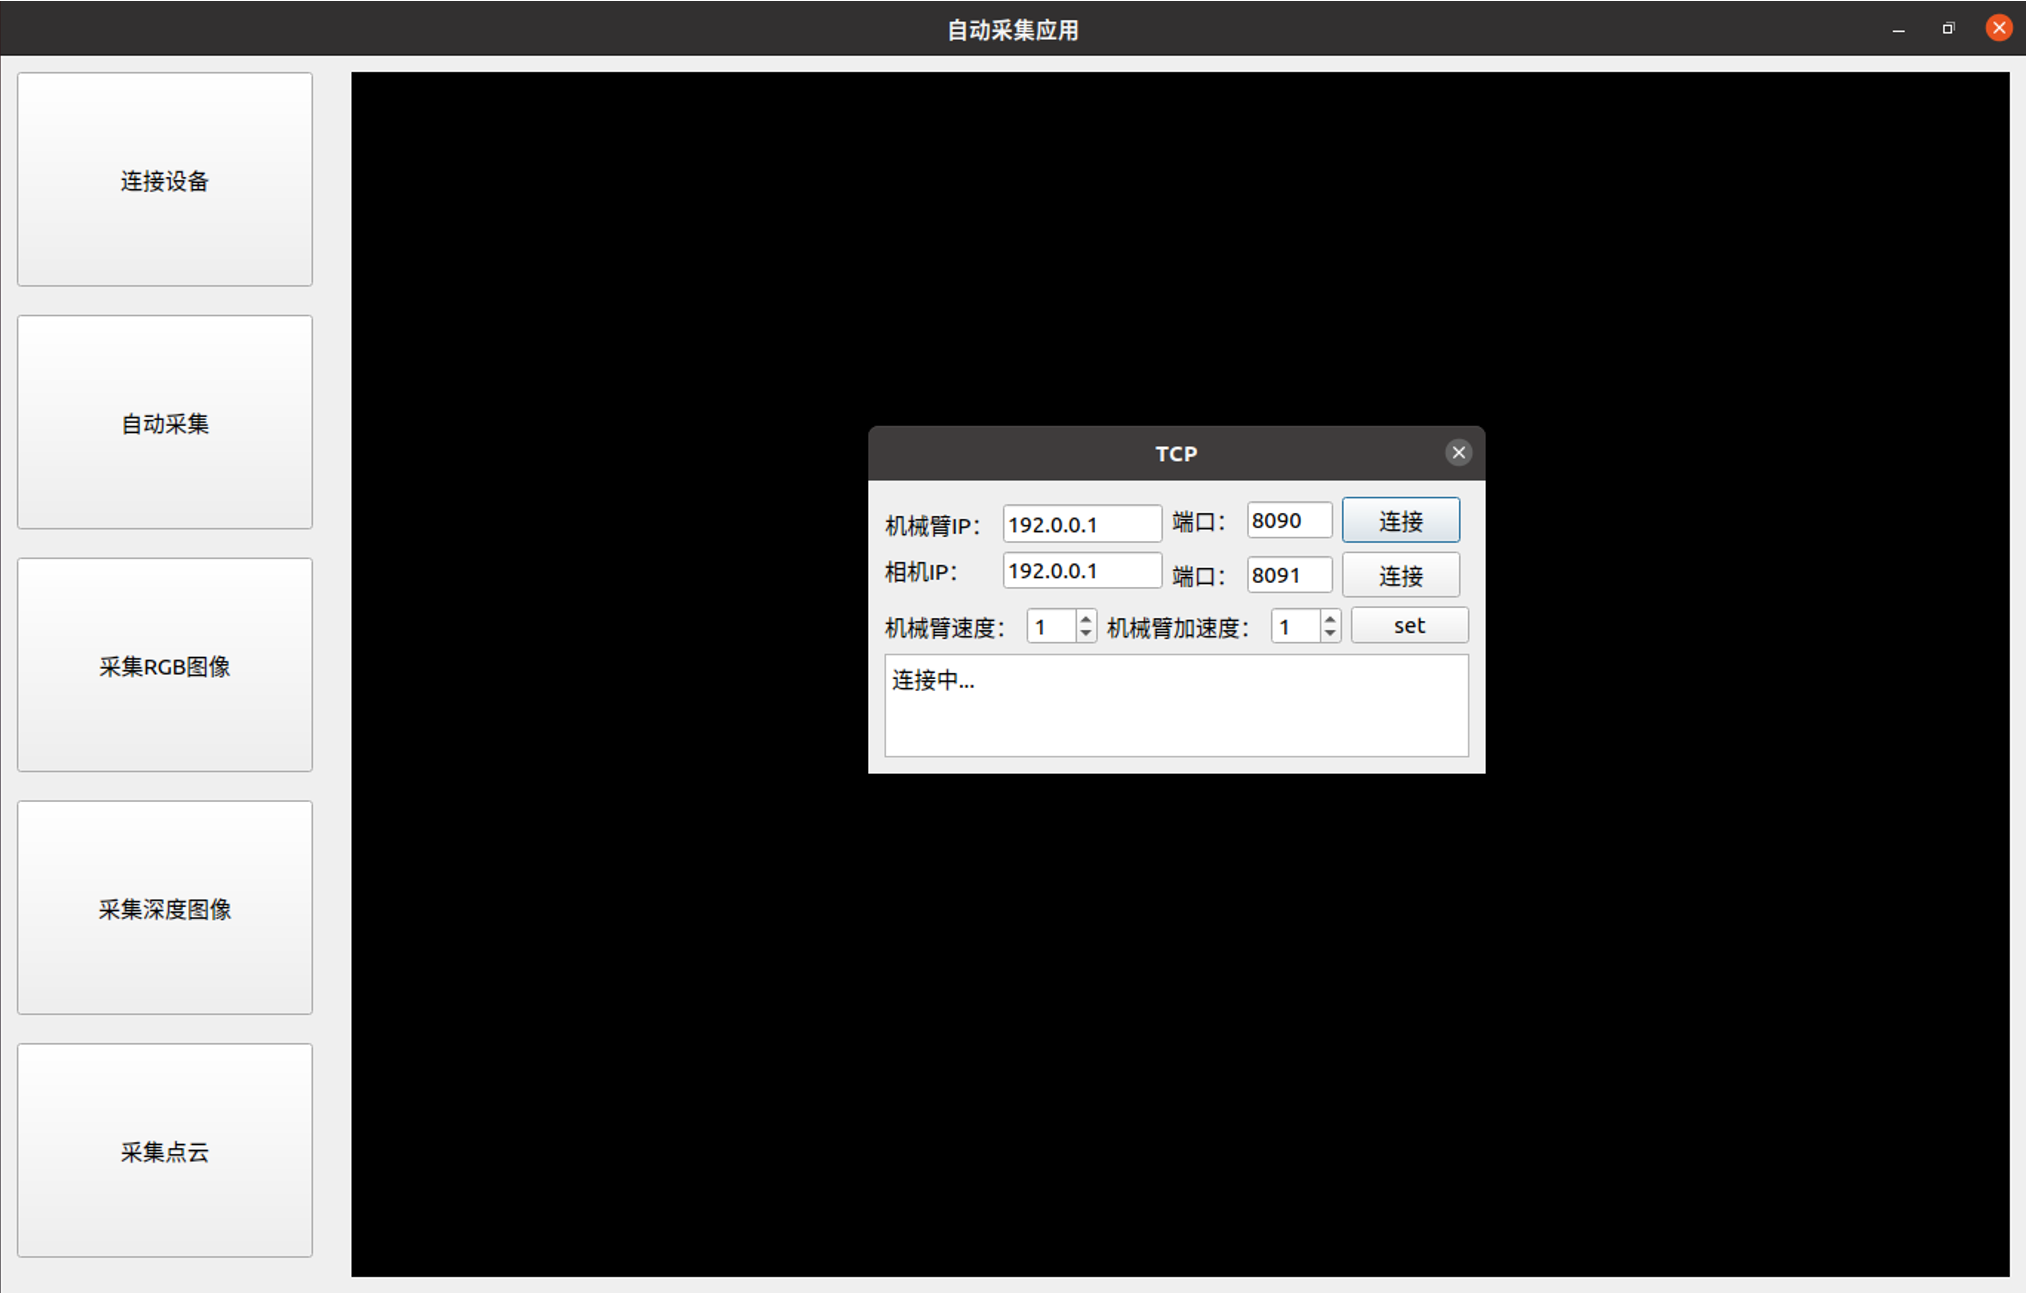
\includegraphics[width=0.75\textwidth]{figures/2/application.png}
  \caption{数据自动采集应用界面}\label{fig:application}
\end{figure}
为了更好地模拟工业实际情况下被检物摆放位置不固定的情况,提高本文缺陷检测实验的效率,本文设计了一个具有可视化交互界面的数据自动采集应用,界面如图\ref{fig:application}所示。这个应用能够一键采集被检对象在指定场景下的数据并打包生成原始数据集,使其可以供后续缺陷检测算法使用。在本文的实验过程中,该应用大大提高了数据采集的效率,并且能够更好地模拟实际工业场景,从而更全面地评估缺陷检测算法的性能。

\begin{figure}[htbp]
  \centering
  \includegraphics[width=0.5\textwidth]{figures/2/capflow.pdf}
  \caption{数据自动采集应用流程图}\label{fig:capflow}
\end{figure}

数据自动采集应用主要由设备连接和数据自动采集两部分构成,流程如图\ref{fig:capflow}所示。其中设备连接部分主要是调用结构光相机和协作机器人提供的SDK中的设备连接API,并使用Qt制作交互界面,供用户输入相机和机器人的IP地址进行握手连接。

数据自动采集部分的核心思路是利用在硬件平台里提到的结构光相机和协作机器人组成的感知硬件系统,通过执行相机采集、回传工控机数据、工控机下达协作机器人关节运动指令、相机再采集的闭环步骤实现多视角数据采集。

其中相机采集步骤,由于梅卡曼德提供的相机SDK中直接输出的是ply格式的无序点云,而本文需要有序点云。因此本文在原SDK的基础上进行了适配开发,重载了导出函数,实现了导出pcd格式有序点云。回传工控机数据步骤主要是对相机采集的数据进行编号并存储至对应文件夹,从而构建包括训练集和测试集的数据集。工控机存储完数据后触发机械臂控制函数,待机械臂运动至目标点后再触发相机采集数据函数。


\section{评价指标}
本文研究目标为图像级缺陷检测,即着眼于算法对正常样本和缺陷样本分类性能。因此本文主要采用ROC
和AUROC作为本文用于评价算法性能的指标。

在测试时,缺陷检测算法的预测结果有表\ref{tab:matrix}所示的四种可能:当测试样本为正常样本,算法预测也为正常样本,即真正例(True Positive,TP);测试样本为正常样本,但算法预测为缺陷样本,即假负例(False Negative,FN);测试样本为缺陷样本,算法预测也为缺陷样本,即真负例(True Negative,TN);测试样本为缺陷样本,但算法预测为正常样本,即假正例(False Positive,FP)。

\begin{table}[htbp]
  \centering
  \caption{缺陷检测混淆矩阵}\label{tab:matrix}
  \begin{tabular}{@{}cccc@{}} \toprule
       &         & \multicolumn{2}{c}{预测值} \\ \cmidrule(r){3-4}
         &        & 正常=1 & 缺陷=0 \\ \midrule
  \multirow{2}{*}{标签值}	& 正常=1 & TP & FN \\
            & 缺陷=0 & FP & TN \\ \bottomrule
   \end{tabular}
  \end{table}

\subsection{ROC曲线}

ROC(The Receiver Operating Characteristic,受试者操作特征曲线)是一种显示分类模型在所有分类阈值下的性能的图表。这条曲线绘制了两个参数:

真正例率TPR (True Positive Rate),即召回率(Recall):
\begin{equation}
  T P R=\frac{T P}{T P+F N}
\end{equation}

假正例率FPR(False Positive Rate)计算公式如下:
\begin{equation}
  F P R=\frac{F P}{F P+T N}
\end{equation}

ROC图表以FPR为横轴,TPR为纵轴,采用不同分类阈值时的(TPR,FPR)作为坐标绘制ROC曲线。


\subsection{AUROC
}


AUROC(Area under the ROC curve,ROC曲线下面积)是用来衡量二分类机器学习算法性能的一种指标。曲线下面积测量的是从 $(0,0)$ 到 $(1,1)$ 之间整个 ROC 曲线以下的整个二维面积。AUC值的范围在$(0,1)$之间,AUC的值越大表明模型分类能力越好。\cite{bradleyUseAreaROC1997} 

\section{本章小结}
本章为后续缺陷检测算法研究搭建了软硬件系统实验平台,首先介绍了本文用于采集数据的的核心硬件设备结构光相机的原理,然后说明了本文搭建实验平台所需的软件环境和硬件设备,并介绍了如何对相机进行标定。此外,为了更好地采集数据,本章还设计了具有交互界面的自动数据采集的应用。在本章最后,介绍了缺陷检测实验所用到的评价指标ROC和AUROC。